%%%%%%%%%%%%%%%%%%%%%%%%%%%%%%%%%%%%%%%%%%%%%%%%%%%%%%%%%%%%%%%%%%%%%%%%%
% Reference: en.wikibooks.org/wiki/LaTeX/Presentations
%
% An example of use of beamer. 
%%%%%%%%%%%%%%%%%%%%%%%%%%%%%%%%%%%%%%%%%%%%%%%%%%%%%%%%%%%%%%%%%%%%%%%%%%

\documentclass[12pt]{beamer}
\usepackage[utf8]{inputenc}

% Theme config
\usetheme{Madrid}
\usecolortheme{seahorse} %beaver for red, seahorse for light blue

% Title information
\title[Convolutional Networks for Breast Cancer]{Segmentation of Breast Cancer Masses in Digital Mammograms: A
Convolutional Network}
\subtitle{Preliminary results}
\author[Cobos, Terashima] {Erick Cobos Tandazo\inst{1} \and Hugo Terashima Marín\inst{1}}
\date[April 2016]{Congreso Multidisciplinario de Investigacion, April 2016}
\institute[Tecnológico de Monterrey]{
	\inst{1} Sistemas Inteligentes \\ Instituto Tecnológico de Monterrey
}
\begin{document}

	\begin{frame}
		\titlepage
	\end{frame}
	% Presentar los objetivos: dar a conocer en lo que hemos trabajado en el grupo de investigación e interesarlos en cancer de mamá y Deep Learning.
	
	%Table of contents
	\begin{frame}
		\frametitle{Table of Contents}
		\tableofcontents
	\end{frame}

	\section{Breast Cancer}
	\begin{frame}
		\frametitle{Why breast cancer?}
		% Cancer es un término que se usa para describir varias enfermedades distintas donde celulas anormales se multiplican sin control produciendo tuimores y eventualmente invadiendo tejido cercano. Las diferentes denominaciones depende del organo donde se genero
		
		Breast cancer is the most commonly diagnosed cancer in women and, besides lung cancer, the deadliest.
		% Cerca de 1 de cada 3 canceres (30%) los cancers diagnosticados en mujeres son cancer de mama. De hecho, 1 de cada 8 mujeres van a ser diagnosticadas con breast cancer.
		% 15% de todos los diagnosticos no pueden ser curados. 
	
		However, survival rate when detected early is close to 100\%
	\end{frame}
	
	
	
	\begin{frame}
		\frametitle{Breast cancer signs}
		\framesubtitle{Microcalcifications and breast masses}
		
		\begin{figure}
			\centering
			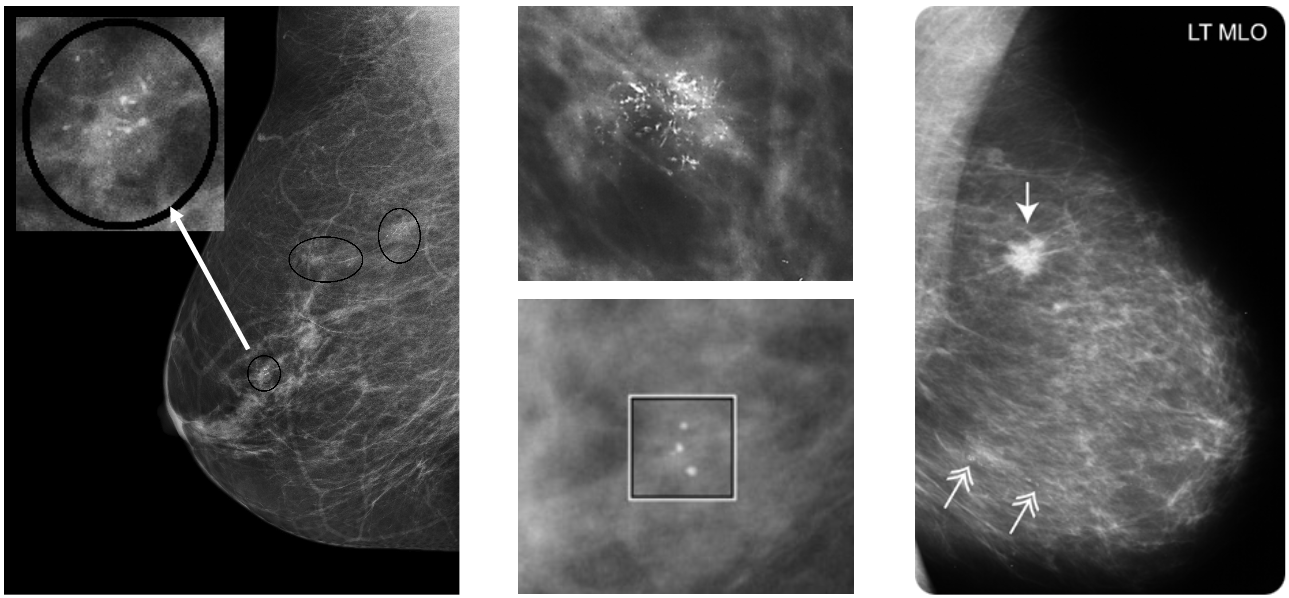
\includegraphics[width = \textwidth]{plots/signs.png}
		\end{figure}
		
		% Mammograms are pictures of the breasta and are currently the recommended screening system
		% Radiologist look primarily for two features: microcalcifications and masses
		% To automate this task. 
	\end{frame}
	
	

	\section{Machine Learning}
	\begin{frame}
		\frametitle{What do we plan to do?}
		% We plan to automate the segementation task
		% Machine learning learns features from data
		% Convnets are one model that does this.
	\end{frame}
	
	\begin{frame}
		\frametitle{Why convolutional networks?}
		Convnets have showed great results in image classification tasks.
		
		Convnets learn which features are important for the classification.
		
		We can use as is to perform image segmentation.

		We don’t need experts to carefully handcraft and select features.


		Cons: Needs processing power, data.
	\end{frame}
	
	\begin{frame}
		\frametitle{Some convnet successes}
		% AlphaGo, Google Photo Recognition, Facebook Tagging, automatic captioning, automatic drone control, clasificación de galaxias, Deep Dream, deep Art (einstein in van gogh, microsoft how old are you
	\end{frame}	
	
	\section{Our work}
	\begin{frame}
		\frametitle{Our work}
		Literature Review

		Obtain and preprocess data set
		
		Design, implement and test a network
		
		Prepare equipment
	
		[In progress] Training the networks
	\end{frame}
	
	\begin{frame}
		\frametitle{Collaboration}
		Apply machine learning to your problems
		
		Solve problems in Machine Learning
		
		Explore new ideas
		%Aplicarlo a imagenes de fmri, o aplicarlo en buscra una forma de representaci	[on comun. 
		%En esto voy atrabajar una vez quetermine este proyecto y probablemente en el doctorado (aunque aun no decido).
	\end{frame}
	
	\begin{frame}
		\frametitle{Thanks!}
		
		\begin{figure}
			\centering
			
\includegraphics[width = 0.25\textwidth]{plots/question.jpg}
		\end{figure}
		
	\end{frame}
\end{document}
